%% FullCourse_10Lecs -- Lecture 4, Topic 4.2: NNs for Value/Policy + Actor-Critic
%% Source: ./archive_pre_split/Lec04_DL_RL_Macro.tex (sections 3-4)
%% Pass B: layer in refinements from
%%         ../../MiniCourse_8hr/Slides/Module2_DL_RL_Macro/M2_T1_VFI_DL.tex
%% Pass B addition: forward reference to Lec05 RL Nutshell (Course_Revision_Plan.md §1F).

%% Shared preamble for the FullCourse_10Lecs topic decks.
%%
%% Each topic .tex \input's this file, then defines its own \title, \date
%% override (if any), \graphicspath, and \begin{document}.
%%
%% Reconstructed verbatim from the inlined copy preserved in
%% Lec10_Case_Studies/Lec10_T8_Case6_DeepRamsey.tex (lines 23-190), which is
%% explicitly annotated there as "from ../shared_preamble.tex, copied verbatim".
%% Base preamble matches MiniCourse_8hr/Slides/shared_preamble.tex; this version
%% additionally provides \sectiondivider, the conceptbox/cautionbox/examplebox/
%% takeawaybox tcolorboxes, and \compacttables used across the split decks.

\documentclass[10pt,english,aspectratio=169]{beamer}

\usepackage{ae,aecompl}
\usepackage[T1]{fontenc}
\usepackage{textcomp}
\usepackage[utf8]{inputenc}
\usepackage{babel}
\usepackage{datetime2}

\setcounter{secnumdepth}{3}
\setcounter{tocdepth}{3}

\usepackage{amsmath, amssymb, amsthm, graphicx}
\usepackage{booktabs, multirow}
\usepackage{tikz}
\usepackage{pgfplots}
\pgfplotsset{compat=1.16}
\usepackage[most]{tcolorbox}
\tcbuselibrary{skins, breakable, theorems}
\usepackage{listings}
\usepackage{xcolor}

\lstset{
  basicstyle=\ttfamily\small,
  keywordstyle=\color{blue!80!black}\bfseries,
  commentstyle=\color{green!50!black}\itshape,
  stringstyle=\color{orange!80!black},
  backgroundcolor=\color{gray!8},
  frame=single,
  rulecolor=\color{gray!40},
  breaklines=true,
  showstringspaces=false,
  numbers=none,
}

\lstdefinestyle{pythonstyle}{
    language=Python,
    basicstyle=\ttfamily\footnotesize,
    keywordstyle=\color{blue!80!black}\bfseries,
    commentstyle=\color{green!50!black}\itshape,
    stringstyle=\color{orange!80!black},
    frame=single,
    breaklines=true,
    showstringspaces=false,
    numbers=left,
    numbersep=5pt,
    numberstyle=\tiny\color{gray},
    backgroundcolor=\color{gray!8},
    rulecolor=\color{gray!40}
}

\ifx\hypersetup\undefined
  \AtBeginDocument{%
    \hypersetup{bookmarks=false,breaklinks=true,pdfborder={0 0 0},colorlinks=true,
      linkcolor=DarkText,urlcolor=RedTitle}%
  }
\else
  \hypersetup{bookmarks=false,breaklinks=true,pdfborder={0 0 0},colorlinks=true,
    linkcolor=DarkText,urlcolor=RedTitle}%
\fi

\makeatletter
\newcommand\makebeamertitle{%
  \begin{frame}[plain]
    \vspace*{1.0cm}
    \centering
    {\usebeamerfont{title}\usebeamercolor[fg]{title}\inserttitle\par}
    \vspace{1.0cm}
    {\usebeamerfont{author}\usebeamercolor[fg]{author}\insertauthor\par}
    \vspace{0.2cm}
    {\usebeamerfont{date}\usebeamercolor[fg]{date}\insertdate\par}
  \end{frame}}%
\AtBeginDocument{%
  \let\origtableofcontents=\tableofcontents
  \def\tableofcontents{\@ifnextchar[{\origtableofcontents}{\gobbletableofcontents}}
  \def\gobbletableofcontents#1{\origtableofcontents}%
}

\usetheme{metropolis}
\usefonttheme{professionalfonts}

\definecolor{LightGray}{RGB}{230,230,230}
\definecolor{RedTitle}{RGB}{0,0,200}
\definecolor{VeryLightGray}{RGB}{245,245,245}
\definecolor{DarkText}{RGB}{0,0,0}

\setbeamercolor{background canvas}{bg=white}
\setbeamercolor{title}{fg=RedTitle}
\setbeamercolor{author}{fg=DarkText}
\setbeamercolor{date}{fg=DarkText}
\setbeamercolor{frametitle}{bg=VeryLightGray,fg=DarkText}
\setbeamercolor{normal text}{fg=DarkText}
\setbeamerfont{title}{size=\large}

\setbeamersize{text margin left=5mm, text margin right=5mm}
\addtobeamertemplate{frametitle}{}{\vspace{-0.5em}}
\newcommand{\reducevspace}{\vspace{-0.5cm}}

% Shared section divider and box styles for split topic decks.
\newcommand{\sectiondivider}[2]{%
\begin{frame}[plain,noframenumbering]
\begin{center}
\vfill
{\Large\textbf{#1}\par}
\vspace{0.35cm}
{\normalsize #2\par}
\vfill
\end{center}
\end{frame}
}

\newtcolorbox{conceptbox}[1][]{
  colback=blue!3,
  colframe=RedTitle!55,
  boxrule=0.35mm,
  arc=1mm,
  left=2mm,
  right=2mm,
  top=1mm,
  bottom=1mm,
  #1
}
\newtcolorbox{cautionbox}[1][]{
  colback=red!3,
  colframe=red!50!black,
  boxrule=0.35mm,
  arc=1mm,
  left=2mm,
  right=2mm,
  top=1mm,
  bottom=1mm,
  #1
}
\newtcolorbox{examplebox}[1][]{
  colback=green!3,
  colframe=green!45!black,
  boxrule=0.35mm,
  arc=1mm,
  left=2mm,
  right=2mm,
  top=1mm,
  bottom=1mm,
  #1
}
\newtcolorbox{takeawaybox}[1][]{
  colback=VeryLightGray,
  colframe=RedTitle!55,
  boxrule=0.35mm,
  arc=1mm,
  left=2mm,
  right=2mm,
  top=1mm,
  bottom=1mm,
  #1
}
\newcommand{\compacttables}{\renewcommand{\arraystretch}{1.15}}

\setbeamertemplate{navigation symbols}{}
\setbeamertemplate{footline}{%
  \hfill%
  \usebeamercolor[fg]{page number in head/foot}%
  \usebeamerfont{page number in head/foot}%
  \insertframenumber\,/\,\inserttotalframenumber\kern1em\vskip2pt%
}

\makeatother

\author{Zhigang Feng}
% "date with time": compile timestamp so each build is identifiable.
\date{\today\ \DTMcurrenttime}


\graphicspath{{./pic/}{../../MiniCourse_8hr/Slides/Module2_DL_RL_Macro/pic/}{../}}

% Suppress the redundant auto-generated metropolis section page; the
% \sectiondivider frames below are the dividers we keep.
\metroset{sectionpage=none}
\usetikzlibrary{positioning,arrows.meta,shapes,calc}
%% Lec04 shared MAP slide: "one map, four acts" recurring diagram.
%% Input this file AFTER ../shared_preamble.tex (needs RedTitle, VeryLightGray,
%% DarkText) and AFTER \usetikzlibrary{positioning,arrows.meta,shapes,calc}.
%% Call \LecFourMap{k} inside a frame, where k in {1,2,3,4} highlights the
%% current act ("you are here") and k = 0 renders the closing reprise with all
%% four acts checked green (used by T4's closing frame).
%% Filename deliberately does NOT match the build glob Lec*_T*.tex, so the build
%% script never tries to compile it standalone.
%%
%% The four acts are the lecture's story: PROBLEM -> SOLVE -> CODE -> TRUST,
%% one running example throughout (the optimal growth model): why grids break,
%% the Bellman route (deep VFI + actor-critic), the Euler route in PyTorch,
%% and structured networks + the validation gate.

\newcommand{\LecFourMap}[1]{%
% Precompute per-box style selectors; TikZ option lists are comma-split before
% TeX conditionals run, so \ifnum must not sit inside a [...] options list.
\ifnum#1=0
  \tikzset{lmapa/.style={lmapdone}, lmapb/.style={lmapdone},
           lmapc/.style={lmapdone}, lmapd/.style={lmapdone}}%
\else
  \tikzset{lmapa/.style={}, lmapb/.style={}, lmapc/.style={}, lmapd/.style={}}%
  \ifnum#1=1 \tikzset{lmapa/.style={lmapcur}}\fi
  \ifnum#1=2 \tikzset{lmapb/.style={lmapcur}}\fi
  \ifnum#1=3 \tikzset{lmapc/.style={lmapcur}}\fi
  \ifnum#1=4 \tikzset{lmapd/.style={lmapcur}}\fi
\fi
\begin{center}
\begin{tikzpicture}[
    act/.style={rectangle, rounded corners, draw=black!60, fill=VeryLightGray,
        minimum width=3.0cm, minimum height=0.95cm, text width=2.9cm,
        align=center, font=\small, text=DarkText},
    lmapcur/.style={draw=RedTitle, very thick, fill=orange!20},
    lmapdone/.style={draw=green!45!black, thick, fill=green!10},
    q/.style={font=\tiny\itshape, text width=3.0cm, align=center, text=black!70},
    barlab/.style={font=\tiny\bfseries, text=black!65},
    sat/.style={rectangle, rounded corners, draw=black!45, dashed, fill=white,
        text width=5.2cm, align=center, font=\tiny, text=black!70,
        minimum height=0.5cm},
    arr/.style={-{Stealth[length=2.2mm]}, thick, gray!60}
]
    % --- four act boxes ---
    \node[act, lmapa] (a1) at (0,0)
        {\textbf{4.1\ \ PROBLEM}\\[1pt] \tiny growth model $\cdot$ curse of dim.};
    \node[act, lmapb] (a2) at (3.6,0)
        {\textbf{4.2\ \ SOLVE}\\[1pt] \tiny deep VFI $\cdot$ actor--critic};
    \node[act, lmapc] (a3) at (7.2,0)
        {\textbf{4.3\ \ CODE}\\[1pt] \tiny Euler loss $\cdot$ PyTorch};
    \node[act, lmapd] (a4) at (10.8,0)
        {\textbf{4.4\ \ TRUST}\\[1pt] \tiny ICNN $\cdot$ validation $\cdot$ lab};
    \draw[arr] (a1) -- (a2);
    \draw[arr] (a2) -- (a3);
    \draw[arr] (a3) -- (a4);
    % --- the student question each act answers ---
    \node[q] at (0,-0.95)    {why do grids break on\\ real macro models?};
    \node[q] at (3.6,-0.95)  {how do neural nets solve\\ the Bellman equation?};
    \node[q] at (7.2,-0.95)  {how do I code it --- loss,\\ networks, training loop?};
    \node[q] at (10.8,-0.95) {can I trust the answer ---\\ and how do I prove it?};
    % --- "you are here" marker above the current act ---
    \ifnum#1=1 \node[font=\scriptsize\bfseries, text=RedTitle] at (0,0.98)
        {you are here\ $\blacktriangledown$};\fi
    \ifnum#1=2 \node[font=\scriptsize\bfseries, text=RedTitle] at (3.6,0.98)
        {you are here\ $\blacktriangledown$};\fi
    \ifnum#1=3 \node[font=\scriptsize\bfseries, text=RedTitle] at (7.2,0.98)
        {you are here\ $\blacktriangledown$};\fi
    \ifnum#1=4 \node[font=\scriptsize\bfseries, text=RedTitle] at (10.8,0.98)
        {you are here\ $\blacktriangledown$};\fi
    \ifnum#1=0 \node[font=\scriptsize\bfseries, text=green!45!black] at (5.4,0.98)
        {all four acts complete};\fi
    % --- bottom band: two solution routes + the audit (the technical spine) ---
    \fill[blue!10]   (-1.55,-1.72) rectangle (5.15,-1.40);
    \fill[green!12]  (5.65,-1.72)  rectangle (8.75,-1.40);
    \fill[orange!16] (9.25,-1.72)  rectangle (12.35,-1.40);
    \node[barlab] at (1.8,-1.56)  {BELLMAN ROUTE\ ($V$, $g$ networks)};
    \node[barlab] at (7.2,-1.56)  {EULER ROUTE\ (FOC residuals)};
    \node[barlab] at (10.8,-1.56) {AUDIT GATE\ (Lab 3A/3B)};
    % --- dashed satellites: where this lecture sits in the course flow ---
    \node[sat] at (1.5,-2.42)
        {\textit{upstream:} Lec03 --- the NN toolkit (architecture, UAT, training, ICNN)};
    \node[sat] at (9.3,-2.42)
        {\textit{downstream:} Lec05 --- the RL theory behind actor--critic; Lec06 --- heterogeneous agents at scale};
\end{tikzpicture}
\end{center}
}


\title[AI for Econ Research]{AI for Economic Research: Dynamic Models, Language, and Agents\\
Lecture 4.2: Deep VFI \& Actor-Critic for Growth}

\begin{document}

\makebeamertitle

%=============================================================================
\begin{frame}{Lecture 4 in One Map}
\textbf{One lecture, four decks, one running example: solve the optimal growth model with deep learning --- pose the problem, solve it two ways, code it, and prove the answer right.}

\LecFourMap{2}

\vspace{0.05cm}
\footnotesize\textit{\textbf{Act 4.2 (here)} solves it the Bellman way: replace the grid with networks for $V$ and $g$, train them on simulated states, and meet actor--critic --- the algorithm Lec.\ 5 T3 formalizes.}
\end{frame}

%=============================================================================
\section{Deep Learning Approach: NNs for Value and Policy Functions}

\sectiondivider{Deep Learning Approach: NNs for Value and Policy Functions}{Replace the grid with networks for $V$ and $g$ --- mesh-free, dimension-robust}

%---------------------------------------
\begin{frame}{The Core Idea: Replace Grids with Neural Networks}
\begin{itemize}
  \item \textbf{Instead of} storing $V(k)$ on a grid, \textbf{approximate} it with a neural network:
    \[
      V(k) \approx \Gamma_{\gamma_v}(k), \qquad g(k) \approx \Gamma_{\gamma_g}(k)
    \]
    where $\gamma_v, \gamma_g$ are network parameters (weights and biases)
  \medskip
  \item \textbf{The analogy to VFI}:
    \begin{enumerate}
      \item Generate states $k \sim D(k)$ from some distribution (replaces grid)
      \item Compute approximate target values or gradients for training
      \item Update $\gamma_v$ or $\gamma_g$ using gradient-based optimization
    \end{enumerate}
  \medskip
  \item \textbf{Why this helps}: Neural networks handle high-dimensional $k$ naturally
    \begin{itemize}
      \item No grid needed --- states are \emph{sampled}
      \item The network generalizes across the state space
      \item Parameters grow polynomially, not exponentially, with dimension
    \end{itemize}
\end{itemize}
\end{frame}

%---------------------------------------
\begin{frame}{Embedding Equilibrium Conditions in Neural Networks}
\begin{itemize}
  \item Neural network approximations can incorporate \textbf{equilibrium conditions} directly:
    \begin{itemize}
      \item \textbf{Feasibility constraints}: Ensure $g(k) \in \mathcal{G}(k)$
        \begin{itemize}
          \item Example: $0 \leq c \leq f(k)$ (can't consume more than output)
        \end{itemize}
      \item \textbf{Market clearing}: $\sum_i c_i = Y$ or asset market clearing
      \item \textbf{Budget constraints}: Household or government budget balance
    \end{itemize}
  \medskip
  \item \textbf{Implementation strategies}:
    \begin{enumerate}
      \item \textbf{Output transformations}: Sigmoid $\to$ bound outputs within feasible range
      \item \textbf{Penalty methods}: Add constraint violation terms to the loss
      \item \textbf{Lagrangian approaches}: Dual variables updated during training
      \item \textbf{Architectural design}: Structure the network so outputs automatically satisfy identities
    \end{enumerate}
  \medskip
  \item Building in economic structure improves convergence and ensures economically meaningful solutions
\end{itemize}
\end{frame}

%---------------------------------------
\begin{frame}{Deep VFI: The Algorithm at a Glance}
\textit{\footnotesize Before the details: the whole loop in one place --- a value step and a policy step, alternated, on sampled states.}

\vspace{0.15cm}
\begin{conceptbox}
\footnotesize
\textbf{Deep Value Function Iteration} --- represent $V\approx\Gamma_{\gamma_v}$, $g\approx\Gamma_{\gamma_g}$; iterate:
\begin{enumerate}\footnotesize
  \item \textbf{Sample} a batch of states $\{k_i\}\sim D(k)$ \quad(no grid)
  \item \textbf{Value step (critic)}: fit $\Gamma_{\gamma_v}$ to the Bellman target
        $\hat V(k)=u(k,g(k))+\beta\,\Gamma_{\gamma_v}\!\bigl(f(k,g(k))\bigr)$ by least squares
  \item \textbf{Policy step (actor)}: improve $\Gamma_{\gamma_g}$ by gradient \emph{ascent} on
        $u(k,g(k))+\beta\,\Gamma_{\gamma_v}\!\bigl(f(k,g(k))\bigr)$
  \item \textbf{Repeat} until $\Gamma_{\gamma_v},\Gamma_{\gamma_g}$ stabilize
\end{enumerate}
\end{conceptbox}
\medskip
\begin{itemize}\footnotesize
  \item Same rhythm as classical VFI --- \emph{evaluate} the current policy, then \emph{improve} it --- but with a \textbf{neural network} instead of traditional function approximation (interpolation, splines), and \textbf{sampled states} instead of a grid.
  \item The next slides unpack each step; the following section recasts the same loop in \textbf{actor-critic} language.
\end{itemize}

\vspace{0.05cm}
{\footnotesize\textit{Expectations over shocks are estimated by Monte-Carlo simulation; that sampling machinery is developed in Lecture~5.}}
\end{frame}

%---------------------------------------
\begin{frame}{Deep VFI vs.\ Classical VFI}
\textit{\footnotesize Same Bellman logic, different machinery --- this is what lets it scale.}

\vspace{0.15cm}
\begin{center}
\compacttables\scriptsize
\begin{tabular}{@{}l l l@{}}
\toprule
 & \textbf{Classical VFI} & \textbf{Deep VFI} \\
\midrule
State space       & fixed grid $\{k_1,\dots,k_N\}$      & sampled batch $k_i\sim D(k)$ \\
Representation    & table / interpolation               & neural network $\Gamma_\gamma(k)$ \\
Value update      & exact $\max_{k'}$ at each grid point & least-squares fit to $\hat V$ \\
Policy            & $\arg\max$ by grid search           & learned policy net (grad.\ ascent) \\
Expectation       & quadrature on a grid                & Monte-Carlo over simulated shocks \\
Cost vs.\ dim $d$ & $N^d$ (curse of dimensionality)     & polynomial in $d$ \\
Convergence       & contraction guarantee (Banach)      & no general guarantee (empirical) \\
\bottomrule
\end{tabular}
\end{center}
\medskip
\begin{itemize}\footnotesize
  \item The trade: \textbf{give up} the exact grid max and the contraction guarantee; \textbf{gain} the ability to scale to high dimensions and to fit scattered, simulated data.
  \item \textbf{Monte-Carlo} supplies the expectations; its details (sampling, exploration, variance) are the subject of \textbf{Lecture~5}.
\end{itemize}
\end{frame}

%---------------------------------------
\begin{frame}{Value Function Update (One-Step Look-Ahead)}
\begin{itemize}
  \item Fix a policy $g^{(n-1)}(k) = \Gamma_{\gamma_g}^{(n-1)}(k)$
  \item The one-step approximation for the value is:
    \[
      \hat{V}(k) = u\bigl(k, g^{(n-1)}(k)\bigr) + \beta\, \Gamma_{\gamma_v}^{(n-1)}\bigl(f(k, g^{(n-1)}(k))\bigr)
    \]
  \item We then solve a \textbf{least squares} problem over the sampling distribution:
    \[
      \min_{\gamma_v^{(n)}} \; \mathbb{E}_{k\sim D(k)}\Bigl[\bigl(\Gamma_{\gamma_v}^{(n)}(k) - \hat{V}(k)\bigr)^2\Bigr]
      \;\approx\; \frac{1}{N_v}\sum_{i=1}^{N_v} \bigl(\Gamma_{\gamma_v}^{(n)}(k_i) - \hat{V}(k_i)\bigr)^2
    \]
    {\footnotesize The empirical average $\tfrac{1}{N_v}\sum_i$ is the \textbf{special case} of $\mathbb{E}_{k\sim D(k)}$ using $N_v$ i.i.d.\ draws $k_i\sim D(k)$.}
  \medskip
  \item \textbf{Key}: States $\{k_i\}$ are \emph{sampled} from distribution $D(k)$, not placed on a grid
  \item This is \textbf{supervised learning}: the ``label'' for each $k_i$ is the Bellman target $\hat{V}(k_i)$
  \item \textbf{Detach the target} so gradients do not flow through $\Gamma_{\gamma_v}^{(n-1)}$ (target-network style update --- crucial for stability)
\end{itemize}
\end{frame}

%---------------------------------------
\begin{frame}{The Role of Value Function in Policy Evaluation}
\begin{itemize}
  \item \textbf{What is $\hat V$?} With policy $g^{(n-1)}$ and value net $\Gamma_{\gamma_v}^{(n-1)}$ held \emph{fixed}, the target
    \[
      \hat V(k) = u\bigl(k,g^{(n-1)}(k)\bigr) + \beta\,\Gamma_{\gamma_v}^{(n-1)}\!\bigl(f(k,g^{(n-1)}(k))\bigr)
    \]
    is \textbf{one Bellman backup} under the current policy: $\hat V = T_{g^{(n-1)}}\Gamma_{\gamma_v}^{(n-1)}$.
  \medskip
  \item \textbf{Why $\hat V \approx V^*$?} At the optimum the Bellman equation holds exactly, $T_{g^*}V^* = V^*$ --- so $V^*$ is a \emph{fixed point} of the backup. Since $T_{g}$ is a $\beta$-contraction,
    \[
      \|\hat V - V^*\| \;\le\; \beta\,\underbrace{\|\Gamma_{\gamma_v}^{(n-1)} - V^*\|}_{\text{value error}} \;+\; \underbrace{\|T_{g^{(n-1)}}V^* - V^*\|}_{\text{policy suboptimality}\,\to\,0}
    \]
  \item Each backup \textbf{shrinks the value error by a factor $\beta$} (plus a term that vanishes as $g^{(n-1)}\to g^*$): fitting $\Gamma_{\gamma_v}^{(n)}$ to $\hat V$ and improving the policy drives $\hat V \to V^*$.
  \medskip
  \item \textbf{The average is over states}: $\mathbb{E}_{k \sim D(k)}[\cdot]$ averages the fit across the \emph{state space} (not over shocks) --- good average fitness on sampled states $\Rightarrow$ a good global approximation.
\end{itemize}
\end{frame}

%---------------------------------------
\begin{frame}{Policy Function Update}
\begin{itemize}
  \item Given the updated value network $\Gamma_{\gamma_v}^{(n)}$, improve the policy by solving:
    \[
      \max_{\gamma_g^{(n)}} \;\; \mathbb{E}_{k\sim D(k)}\Bigl[ u\bigl(k, \Gamma_{\gamma_g}^{(n)}(k)\bigr) + \beta\, \Gamma_{\gamma_v}^{(n)}\bigl(f(k, \Gamma_{\gamma_g}^{(n)}(k))\bigr) \Bigr]
    \]
  \item This is \textbf{gradient ascent} on the neural network parameters:
    \[
      \gamma_g^{(n)} = \gamma_g^{(n-1)} + \alpha \cdot \nabla_{\gamma_g} J(\gamma_g)\Big|_{\gamma_g = \gamma_g^{(n-1)}}
    \]
  \medskip
  \item \textbf{Two roles of the gradient}:
    \begin{enumerate}
      \item \textbf{Direction}: $\nabla_{\gamma_g} J$ tells us \emph{which direction} in parameter space improves the objective
      \item \textbf{Magnitude}: Combined with learning rate $\alpha$, determines \emph{how far} we move
    \end{enumerate}
  \medskip
  \item In practice, optimizers like Adam adaptively adjust step sizes for faster and more stable convergence
\end{itemize}
\end{frame}

%---------------------------------------
\begin{frame}{Choosing the Sampling Distribution $D(k)$}
\begin{itemize}
  \item The distribution $D(k)$ determines \emph{where} we evaluate the approximation
  \medskip
  \item \textbf{Common choices}:
    \begin{itemize}
      \item \textbf{Uniform}: Simple, but wastes capacity on unlikely states
      \item \textbf{Stationary distribution}: Focuses on states the economy actually visits
      \item \textbf{Importance sampling}: Targets high-uncertainty or high-value regions
    \end{itemize}
  \medskip
  \item \textbf{Stationary distribution approach}:
    \begin{enumerate}
      \item Simulate the economy under current policy for many periods
      \item Wait until the state converges to its ergodic distribution
      \item Draw training points from that distribution
    \end{enumerate}
  \medskip
  \item \textbf{Benefits}: Sample efficiency (focus on what matters), faster convergence, no need for a handcrafted grid
  \item \textbf{Limitation}: Rare but important events (tail risks) may be under-represented
\end{itemize}
\end{frame}

%---------------------------------------
\begin{frame}{Where to Sample? Uniform vs.\ Stationary $D(k)$}
\textit{\footnotesize One-sector stochastic growth: the economy spends almost all its time near the ergodic mean $k_{ss}$ --- so that is where the approximation must be accurate.}

\vspace{0.1cm}
\begin{columns}
  \begin{column}{0.57\textwidth}
    \centering
    \begin{tikzpicture}[scale=0.92, transform shape,
      dot/.style={circle, fill, inner sep=0pt, minimum size=2.3pt}]
      \draw[->,thick] (0,0) -- (6.5,0) node[right,font=\scriptsize] {$k$};
      \draw[->,thick] (0,0) -- (0,3.1) node[above,font=\scriptsize] {$D(k)$};
      % ergodic (stationary) density, peaked near k_ss
      \draw[thick, RedTitle!70] plot[smooth] coordinates
        {(0.4,0.05) (1.2,0.2) (2.0,0.7) (2.7,1.6) (3.4,2.5) (4.1,1.9) (4.8,0.9) (5.5,0.3) (6.1,0.08)};
      \node[RedTitle!70,font=\scriptsize] at (4.9,2.35) {ergodic density};
      \draw[dashed,gray] (3.4,0) -- (3.4,2.5);
      \node[font=\scriptsize] at (3.4,-0.28) {$k_{ss}$};
      % stationary samples: clustered under the peak
      \foreach \x/\y in {2.6/0.35, 2.9/0.75, 3.1/0.3, 3.3/1.0, 3.4/0.5, 3.5/1.4, 3.6/0.25, 3.7/0.85, 3.9/0.4, 4.1/0.6, 3.2/0.2, 3.8/1.1, 4.3/0.3, 3.0/0.5, 2.75/0.2}
        \node[dot, blue!75] at (\x,\y) {};
      \node[blue!75!black,font=\scriptsize,anchor=west] at (1.9,1.8) {stationary};
      % uniform samples: even along the axis
      \foreach \x in {0.45,1.05,...,6.05}
        \node[dot, orange!90] at (\x,-0.6) {};
      \node[orange!80!black,font=\scriptsize,anchor=west] at (0.0,-1.0) {uniform (even in $k$): most points land where the economy never is};
    \end{tikzpicture}
  \end{column}
  \begin{column}{0.43\textwidth}
    \footnotesize
    \begin{itemize}
      \item \textbf{Uniform} (orange): spends half its points on low-$k$ states the economy almost never visits --- wasted capacity.
      \item \textbf{Stationary} (blue): simulate the model forward, keep the ergodic draws --- points land where accuracy matters.
      \item \textbf{Tails}: rare high-/low-$k$ events are under-sampled --- add a few importance-sampled draws if they matter (e.g.\ disaster risk).
    \end{itemize}
  \end{column}
\end{columns}
\end{frame}


%---------------------------------------
\begin{frame}{Why Not Chebyshev Here?}
\begin{itemize}
  \item Chebyshev and finite-element methods must approximate over the \emph{entire} domain
  \item As dimensionality grows, covering the entire domain becomes infeasible
  \medskip
  \item \textbf{Stationarity-based sampling} zooms in on the \emph{likely} region of interest
  \medskip
  \item \textbf{Possible concerns and remedies}:
    \begin{itemize}
      \item \textbf{Rare but important events}: Combine stationary sampling with targeted sampling of rare states (importance sampling)
      \item \textbf{Multiple steady states}: A single stationary distribution might miss transient states
      \item \textbf{Out-of-distribution robustness}: Conduct stress tests separately
    \end{itemize}
  \medskip
  \item The combination of \textbf{Monte Carlo sampling} (generates the right data in relevant states) and \textbf{neural networks} (fits irregular, mesh-free data) is the key synergy
\end{itemize}
\end{frame}

%---------------------------------------
\begin{frame}{Bias-Variance Tradeoff: One-Step vs.\ Multi-Step}
\begin{itemize}
  \item \textbf{One-step} ($T_{\text{sim}} = 1$):
    \[
      \hat{V}(k_i) = u\bigl(k_i, g(k_i)\bigr) + \beta\, \Gamma_{\gamma_v}(k_{i,1})
    \]
    \begin{itemize}
      \item[$+$] Easy to implement, low variance
      \item[$-$] High bias if $V(\cdot)$ approximation is poor
    \end{itemize}
  \medskip
  \item \textbf{$T_{\text{sim}}$-step return}:
    \[
      \hat{V}(k_i) = \sum_{t=0}^{T_{\text{sim}}-1} \beta^t\, u(k_{i,t}, g(k_{i,t})) + \beta^{T_{\text{sim}}}\, \Gamma_{\gamma_v}(k_{i,T_{\text{sim}}})
    \]
    \begin{itemize}
      \item[$+$] Lower bias: uses actual simulated rewards over multiple steps
      \item[$-$] Higher variance: simulated paths can vary significantly
    \end{itemize}
  \medskip
  \item \textbf{In practice}: Choose $T_{\text{sim}}$ to balance bias vs.\ variance (typical values $T_{\text{sim}} = 30$--$50$)
\end{itemize}
\end{frame}

%=============================================================================
\section{Actor-Critic Algorithm for the Growth Model}

\sectiondivider{Actor-Critic Algorithm for the Growth Model}{Two networks teach each other: the critic scores, the actor improves (Lec.\ 5 formalizes)}
% Note: We develop the full RL theory (Monte Carlo, TD, actor-critic)
% in Lecture 5. Here we apply the actor-critic idea to the growth model.

%---------------------------------------
\begin{frame}{Why Actor-Critic? The Optimization Bottleneck}
\textit{\footnotesize We apply the actor-critic \emph{idea} here as a concrete solver for the optimal-growth model; the full RL theory (MDPs, Monte Carlo, TD, on-/off-policy actor-critic) is developed in Lecture~5.}

\begin{itemize}
  \item \textbf{Classical VFI} requires solving $\max_{k'} Q(k, k')$ at every state
  \item When $Q$ is represented by a neural network (non-convex), this inner maximization is expensive and unreliable
  \medskip
  \item \textbf{The actor-critic solution}: Use \emph{two} networks to avoid the inner max:
    \begin{enumerate}
      \item \textbf{The Actor (Policy Net $\pi$)} --- ``The Doer''
        \begin{itemize}
          \item Input: state $k$ $\to$ Output: action $k'$ directly
          \item \emph{Avoids} the expensive maximization step
        \end{itemize}
      \item \textbf{The Critic (Value Net $V$)} --- ``The Judge''
        \begin{itemize}
          \item Input: state $k$ $\to$ Output: estimated value $V(k)$
          \item Minimizes the \textbf{Bellman residual} (prediction error)
        \end{itemize}
    \end{enumerate}
  \medskip
  \item The actor proposes actions; the critic evaluates them; both improve iteratively
\end{itemize}
\end{frame}

%---------------------------------------
\begin{frame}{Mapping Macroeconomics to Reinforcement Learning}
\vspace{-0.3cm}
To apply RL, we translate economic models into the standard tuple $(S, A, P, R, \gamma)$:

\vspace{0.2cm}
\begin{table}[]
\centering
\renewcommand{\arraystretch}{1.4}
\scriptsize
\begin{tabular}{l | l | l}
\textbf{RL Concept} & \textbf{Economic Equivalent} & \textbf{Note} \\
\hline
\textbf{Agent} & Household / Firm & The optimizer \\
\hline
\textbf{Environment} & Constraints \& Prices & The rules of the game \\
\hline
\textbf{State ($S$)} & $(k, z, \Delta)$ & Wealth, shocks, \textbf{distribution} \\
\hline
\textbf{Action ($A$)} & $c, i, l$ & Consumption, investment \\
\hline
\textbf{Transition ($P$)} & $k' = (1-\delta)k + i$ & \textbf{Micro}: Known perfectly \\
& $\Delta' = H(\Delta)$ & \textbf{Macro}: Often unknown/intractable \\
\hline
\textbf{Reward ($R$)} & $u(c)$ & Period utility \\
\hline
\textbf{Discount ($\gamma$)} & $\beta$ & Time preference \\
\end{tabular}
\end{table}

\vspace{0.2cm}
\textbf{The synergy}: RL handles the complexity of the macro transition $\Delta' = H(\Delta)$ by simply \emph{simulating} it, without needing to derive the law of motion explicitly
\end{frame}

%---------------------------------------
\begin{frame}{Actor-Critic Algorithm (Preview --- full treatment in Lec05 T3)}
We use actor-critic here as a \emph{solver} for the growth-model Bellman equation. The MDP framing $(S, A, P, R, \gamma)$, the policy gradient theorem, and the full algorithm family come in Lec05.

\vspace{0.1cm}
\begin{columns}
  \begin{column}{0.54\textwidth}
    \footnotesize
    \begin{enumerate}
      \item \textbf{Initialize}: $\pi_\theta^{(0)}$ ($\equiv \Gamma_{\gamma_g}^{(0)}$), $V_\phi^{(0)}$ ($\equiv \Gamma_{\gamma_v}^{(0)}$)
      \item \textbf{Critic update} ($V_\phi$):
        \begin{itemize}\footnotesize
          \item Data $\{k_i, \hat{V}(k_i)\}$ via $T_{\text{sim}}$-step MC
          \item $\min_{\phi^{(n)}} \mathbb{E}_{k\sim D(k)}\big[(V_\phi^{(n)}(k) - \hat{V}(k))^2\big]$
        \end{itemize}
      \item \textbf{Actor update} ($\pi_\theta$):
        \begin{itemize}\footnotesize
          \item Sample states $\{k_i\}$ (stationary dist.)
          \item $\max_{\theta^{(n)}} \mathbb{E}_{k\sim D(k)}\big[u + \beta\, V_\phi^{(n)} \circ f\big]$
        \end{itemize}
      \item \textbf{Check convergence}; repeat until $\pi_\theta, V_\phi$ stabilize.
    \end{enumerate}
  \end{column}
  \begin{column}{0.46\textwidth}
    \centering
    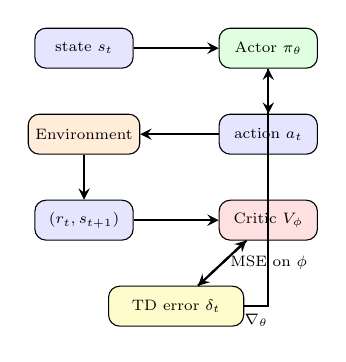
\begin{tikzpicture}[scale=0.78, transform shape,
      box/.style={rectangle,draw,rounded corners,minimum width=1.6cm,minimum height=0.65cm,align=center,font=\scriptsize},
      arr/.style={->,thick,>=stealth}
    ]
      \node[box,fill=blue!10] (state) at (0,2) {state $s_t$};
      \node[box,fill=green!12] (actor) at (3,2) {Actor $\pi_\theta$};
      \node[box,fill=blue!10] (act) at (3,0.6) {action $a_t$};
      \node[box,fill=orange!15] (env) at (0,0.6) {Environment};
      \node[box,fill=blue!10] (rew) at (0,-0.8) {$(r_t, s_{t+1})$};
      \node[box,fill=red!12] (critic) at (3,-0.8) {Critic $V_\phi$};
      \node[box,fill=yellow!20,minimum width=2.2cm] (td) at (1.5,-2.2) {TD error $\delta_t$};

      \draw[arr] (state) -- (actor);
      \draw[arr] (actor) -- (act);
      \draw[arr] (act) -- (env);
      \draw[arr] (env) -- (rew);
      \draw[arr] (rew) -- (critic);
      \draw[arr] (critic) -- (td);
      \draw[arr] (td) -| node[pos=0.25,below,font=\scriptsize]{$\nabla_\theta$} (actor);
      \draw[arr,dashed] (td) -- node[right,font=\scriptsize]{MSE on $\phi$} (critic);
    \end{tikzpicture}

    \vspace{0.05cm}
    {\scriptsize\textit{Actor proposes; Critic judges; TD error updates both.}}
  \end{column}
\end{columns}

\vspace{0.1cm}
{\footnotesize\textit{Lec05 T3 unpacks this as an algorithm family --- full pseudocode, policy-gradient theorem, A2C / PPO / DDPG / SAC variants, and convergence theory.}}
\end{frame}

%---------------------------------------
\begin{frame}{Addressing the Infinite Horizon}
\textbf{The tension}: Macro models maximize over an infinite horizon ($\sum_{t=0}^\infty \beta^t u_t$), but Monte Carlo simulations are always finite.

\vspace{0.3cm}
\textbf{The solution: Bootstrapping}
\begin{itemize}
  \item We don't need to simulate to infinity
  \item We use the \textbf{estimated value function} (Critic) as a proxy for the infinite future:
    \[
      \text{Total Value} \approx \underbrace{\sum_{t=0}^{T-1} \beta^t u_t}_{\text{Simulated rewards}} + \beta^T \underbrace{\hat{V}(s_T)}_{\text{Learned proxy for } \sum_{t=T}^\infty}
    \]
  \medskip
  \item This allows learning infinite-horizon policies using only short simulation rollouts
  \item The Critic improves over time, making the bootstrap estimate more accurate
\end{itemize}
\end{frame}

%---------------------------------------
\begin{frame}{Monte Carlo and Uncertainty}
\begin{itemize}
  \item When the model includes \textbf{stochastic shocks}, the future state evolves randomly
  \item Enumerating all possible future states or integrating over a high-dimensional shock space quickly becomes infeasible (another curse of dimensionality)
  \medskip
  \item \textbf{Monte Carlo simulation} circumvents this:
    \begin{itemize}
      \item Generate a large sample of realized state-and-shock paths
      \item Compute empirical averages to approximate expectations
      \item No need to explicitly deal with the full distribution
    \end{itemize}
  \medskip
  \item \textbf{In practice}:
    \begin{itemize}
      \item Choose $T_{\text{sim}}$ to balance bias vs.\ variance
      \item Use parallel or GPU-based Monte Carlo for large simulation demands
      \item Combine with importance sampling if rare shocks are of interest
    \end{itemize}
\end{itemize}
\end{frame}

%---------------------------------------
\begin{frame}{Advantage I: Flexible Function Approximation}
\begin{itemize}
  \item \textbf{Old way --- Structured grids}:
    \begin{itemize}
      \item Requires tensor product grids or sparse grids (Smolyak)
      \item Adding one state variable \emph{multiplies} the grid size
    \end{itemize}
  \medskip
  \item \textbf{New way --- Neural networks}:
    \begin{itemize}
      \item Universal approximators: can represent any continuous function
      \item Parameter count grows linearly/polynomially with dimension, \emph{not} exponentially
      \item Can handle high-dimensional states (entire shock histories, fine-grained distributions) that break grid-based methods
    \end{itemize}
  \medskip
  \item \textbf{Result}: Models that were previously intractable become solvable
\end{itemize}
\end{frame}

%---------------------------------------
\begin{frame}{Advantage II: The ``Mesh-Free'' Synergy}
Why is the combination of \textbf{Monte Carlo} and \textbf{deep learning} so powerful?

\begin{itemize}
  \item \textbf{Monte Carlo simulation} produces a ``cloud'' of points concentrated in the \textbf{ergodic set} (economically relevant states)
    \begin{itemize}
      \item Traditional interpolators (Chebyshev, splines) require \textbf{structured node sets} (tensor or sparse grids) and degrade on scattered, clustered, high-dimensional Monte-Carlo data --- the curse of dimensionality
    \end{itemize}
  \medskip
  \item \textbf{Neural networks are ``mesh-free''}:
    \begin{itemize}
      \item They do not require a grid
      \item They simply minimize error on \emph{whatever} points you give them
    \end{itemize}
  \medskip
  \item \textbf{Conclusion}: MC generates the \emph{right data} (relevant states), and DL is the \emph{right tool} to fit that irregular data
\end{itemize}
\end{frame}

%--- (Advantage III: Hardware Acceleration and Bridge-to-Lec05 slides removed per review) ---

%=============================================================================
% House-style bridge closer (matches Lec05/Lec09): restate the act, hand off.
\begin{frame}{Bridge: Two Networks Solved It --- Can One Loss Do It Too?}
\textbf{Act 4.2 solved the model the Bellman way: a critic network for $V$, an actor network for $g$, trained on simulated states --- mesh-free exactly where grids exploded.}

\vspace{0.25cm}
\begin{itemize}
  \item Monte Carlo supplies the right data (the ergodic set); neural networks are the right fitter for that scattered, high-dimensional cloud.
  \item \textbf{Next (4.3):} the supervised-learning route --- turn the Euler equation's first-order condition into a loss and minimize residuals directly, then implement everything in PyTorch.
\end{itemize}

\vspace{0.3cm}
\begin{center}
\footnotesize\textit{Arc: 4.1 PROBLEM (growth model $+$ curse) $\;\to\;$ \textbf{4.2 SOLVE} (deep VFI $+$ actor--critic) $\;\to\;$ 4.3 CODE (Euler $+$ PyTorch) $\;\to\;$ 4.4 TRUST (structure $+$ validation).}
\end{center}
\end{frame}

\end{document}
